%Capítulo 1 - Introducción
\chapter{Introducción}
\label{chap:1}

\section{Motivación y objetivo general}
\label{sec:mot}

En la actualidad, se está desarrollando una revolución digital que permite que cualquier organización, empresa,
o incluso los individuos posean acceso constante a sistemas informáticos. Estos sistemas poseen un valor fundamental
para el desarrollo de las tareas diarias por lo que es esencial mantenerlos eficientes, seguros y evitar posibles
errores entre el trabajo esperado y el realmente obtenido.

El acceso masivo a sistemas informáticos genera grandes volúmenes de información, lo que hace que sea muy importante
la manera en que se almacena, accede y analiza dicha información, con el fin de poder generar conocimiento,
descubrir y optimizar procesos a partir de ella de manera eficiente. 
Estos objetivos han generado mucho interés en áreas como \textit{datos masivos} -\textit{Big Data}-,
\textit{minería de datos} -\textit{Data Mining}- o \textit{minería de procesos} -\textit{Process Mining}-~\cite{Rozi07,AalstBook}.
Estas áreas presentan diferentes técnicas y herramientas que permiten manejar la desmesurada catarata de datos.
%%%el problema que existe con estas técnicas es que muchas de ellas, asumen la existencia de un modelo formal
%%%del sistema o proceso a analizar para poder ser aplicadas y, en la práctica, esta especifiación formal es mayormente inexistente.

Particularmente, en el ámbito de la gestión de procesos de negocios y sistemas de información, donde los procesos son 
responsables del correcto funcionamiento del sistema, los usuarios finales y analistas desean obtener
detalles relacionados a estos procesos que les faciliten al entendimiento del proceso observado.
Contar con un modelo claro y simple permite una mejor comprehensión del sistema 
subyacente y posibilita además, utilizar sobre él diferentes técnicas con el objetivo de optimizar
el flujo general del sistema~\cite{Aalst2012}.
La minería de procesos utiliza \textit{logs} de ejecución y diferentes técnicas con el objetivo de descubrir,
analizar y extender modelos formales del proceso revelando el comportamiento real de un sistema~\cite{AalstBook}.
Específicamente la minería de procesos puede dividirse en tres grandes campos: \textit{descubrimiento de procesos},
\textit{validación de procesos} y \textit{mejora de modelos}~\cite{Aalst2004,AalstBook,FahlandA15}.

El primero de ellos, \textit{descubrimiento de procesos} -\textit{process discovery}- consiste
en una técnica de aprendizaje para la generación de un modelo formal que represente el comportamiento
subyacente a un conjunto de \textit{logs} provenientes del proceso real.
El descubrimiento de procesos se presenta como un problema complejo ya que 
el modelo generado debe considerar cuatro dimensiones de calidad opuestas entre sí:
\emph{adecuado} (referida a la habilidad del modelo de reproducir las trazas del log),
\emph{precisión} (referida a la trazas por fuera del log que acepta el modelo),
\emph{generalización} (referida a la capacidad del modelo de representar trazas del sistema que no han sido observadas aún en el log) y
\emph{simplicidad} (referida a la búsqueda de un modelo con la menor complejidad posible)~\cite{BuijsvDBAalst,Aalst2012}.

La mayor parte de las técnicas propuestas dentro del descubrimiento de procesos, asumen únicamente información
positiva como entrada del procedimiento, i.e. la entrada está formada por comportamientos que el modelo debe 
incluir. Sin embargo, existe la posibilidad de mejorar este comportamiento si se considera además información 
adicional. Por ejemplo, si se considera la frecuencia con que ocurre de cada traza, se puede realizar un análisis
ponderado de manera de modelar únicamente aquellos patrones más usuales~\cite{GuntherA07,WeijtersR11,LeemansFA13}.

Existen algunas pocas técnicas que consideran el problema de descubrimiento de procesos como una tarea de
aprendizaje supervisado; es decir, considerando las ejecuciones reales del proceso como información positiva, 
pero incorporando además \emph{información negativa}, considerando está última como comportamientos prohibidos 
del sistema que no deben formar parte del modelo formal. Este tipo de información puede ser crucial para 
obtener un buen modelo que sea representativo del proceso real~\cite{Ferreira2006,Lamma2007,Lamma2008,alberti2008verifiable,Goedertier2009}.

Considerar información negativa, como parte del algoritmo de descubrimiento puede generar grandes beneficios ya que
se puede permitir una simplificación y/o una generalización controlada del modelo restringiendo los procesos de 
manera que no incluya las trazas prohibidas


Una buena medida de la simplicidad de un modelo puede obtenerse, a simple vista, a partir de su representación gráfica.
La visualización del modelo es esencial para cualquier técnica de minería de procesos, para que el resultado sea amigable
y de fácil acceso para los usuarios. Algunos algoritmos de descubrimiento generan modelos muy expresivos
pero que no son intuitivos o son de difícil manejo para un uso real (conocidos como modelos spaghetti)~\cite{AalstSP11}. 
Por este motivo, es importante aplicar técnicas de simplificación y generalización a los modelos resultantes,
de manera de obtener un modelo que además de preciso sea útil.

\begin{example}
    \begin{figure}[H]
        \centering
        \subbottom[\label{sfig:mot.1}$N_1$]{\scalebox{.9}{\begin{tikzpicture}

  \node[tplace] (p0) at (-.5,0) {};
  \node[tplace] (p0') at (.5,0) {};
  \node[transition] (x) at (0,-1) {$a$};
  \node[tplace] (p1) at (0,-2) {};
  \node[transition] (y) at (0,-3) {$b$};
  \node[tplace] (p3) at (1.25,-1) {};
  \node[transition] (z) at (1.25,-2) {$c$};
  \node[tplace] (p4) at (1.25,-3) {};
  \node[tplace] (p5) at (-1,-3) {};
        
  \node[] (t) at (p0) {6};
  \node[] (t) at (p0') {1};
  \node[] (t) at (p3) {2};
  \node[] (t) at (p5) {3};
      
  \draw[style={->,>=triangle 45}] (p0) edge node[right,yshift=1.25mm,xshift=-.75mm]{\scriptsize 3} (x);
  \draw[style={->,>=triangle 45}] (p0') to (x);
  \draw[style={->,>=triangle 45}] (x) to (p1);    
  \draw[style={->,>=triangle 45}] (p1) to (y);      
  \draw[style={->,>=triangle 45},bend left=30] (y) edge node[left]{\scriptsize 2} (p0);
  \draw[style={->,>=triangle 45},bend right=30] (y) to (p0');
  
  \draw[style={->,>=triangle 45}] (p3) to (z);      
  \draw[style={->,>=triangle 45}] (p1) to (z);      
  \draw[style={->,>=triangle 45}] (z) to (p4);

  \draw[style={->,>=triangle 45}] (p5) to (y);

%\node[] (name) at (.5,-4) {$N_1$};
  
\end{tikzpicture}
}}
        \hspace{10mm}
        \subbottom[\label{sfig:mot.2}$N_2$]{\scalebox{.9}{\begin{tikzpicture}

  \node[tplace] (p0) at (-.5,0) {};
  \node[tplace] (p0') at (.5,0) {};
  \node[transition] (x) at (0,-1) {$a$};
  \node[tplace] (p1) at (0,-2) {};
  \node[transition] (y) at (0,-3) {$b$};
  \node[tplace] (p3) at (1.25,-1) {};
  \node[transition] (z) at (1.25,-2) {$c$};
  \node[tplace] (p4) at (1.25,-3) {};
  \node[tplace] (p5) at (-1,-3) {};
        
  \node[] (t) at (p0) {2};
  \node[] (t) at (p0') {1};
  \node[] (t) at (p3) {2};
  \node[] (t) at (p5) {3};
    
  \draw[style={->,>=triangle 45}] (p0) to (x);
  \draw[style={->,>=triangle 45}] (p0') to (x);
  \draw[style={->,>=triangle 45}] (x) to (p1);    
%  \draw[style={->,>=triangle 45}] (p1) to (z);      
  \draw[style={->,>=triangle 45}] (p1) to (y);      
  \draw[style={->,>=triangle 45},bend left=30] (y) to (p0);
  \draw[style={->,>=triangle 45},bend right=30] (y) to (p0');

  \draw[style={->,>=triangle 45}] (p3) to (z);      
  \draw[style={->,>=triangle 45}] (z) to (p4);

  \draw[style={->,>=triangle 45}] (p5) to (y);


  %\node[] (name) at (.5,-4) {$N_2$};

\end{tikzpicture}
}}
        \hspace{10mm}
        \subbottom[\label{sfig:mot.3}$N_3$]{\scalebox{.9}{\begin{tikzpicture}

  \node[tplace] (p0) at (-.5,0) {};
  \node[tplace] (p0') at (.5,0) {};
  \node[transition] (x) at (0,-1) {$a$};
  \node[tplace] (p1) at (0,-2) {};
  \node[transition] (y) at (0,-3) {$b$};
  \node[tplace] (p3) at (1.25,-1) {};
  \node[transition] (z) at (1.25,-2) {$c$};
  \node[tplace] (p4) at (1.25,-3) {};
  \node[tplace] (p5) at (-1,-3) {};
        
  \node[] (t) at (p0) {2};
  \node[] (t) at (p0') {1};
  \node[] (t) at (p3) {2};
  \node[] (t) at (p5) {3};
    
  \draw[style={->,>=triangle 45}] (p0) to (x);
  \draw[style={->,>=triangle 45}] (p0') to (x);
  \draw[style={->,>=triangle 45}] (x) to (p1);    
  \draw[style={->,>=triangle 45}] (p1) to (z);      
  \draw[style={->,>=triangle 45}] (p1) to (y);      
  \draw[style={->,>=triangle 45},bend left=30] (y) to (p0);
  \draw[style={->,>=triangle 45},bend right=30] (y) to (p0');

  \draw[style={->,>=triangle 45}] (p3) to (z);      
  \draw[style={->,>=triangle 45}] (z) to (p4);

  \draw[style={->,>=triangle 45}] (p5) to (y);


  %\node[] (name) at (.5,-4) {$N_3$};

\end{tikzpicture}
}}
        \hspace{10mm}
        \subbottom[\label{sfig:mot.4}]{\scalebox{.9}{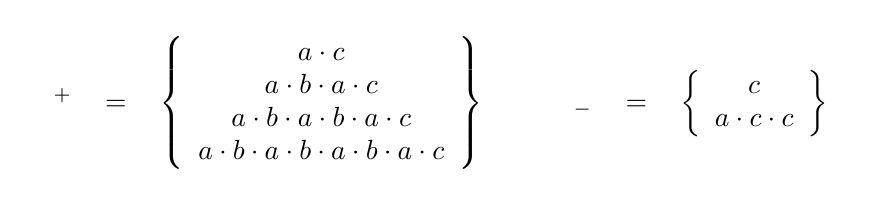
\begin{tikzpicture}

\node[] (logs) at (0,0) {

\begin{tabular}{rcl}
  $\pmlog^+$ & = &
  $\left \{
  \begin{array}{c}
  a \cdot c \\
  a \cdot b \cdot a \cdot c \\
  a \cdot b \cdot a \cdot b \cdot a \cdot c \\
  a \cdot b \cdot a \cdot b \cdot a \cdot b \cdot a \cdot c \\
  \end{array}
  \right \}$
\end{tabular}  
\hspace{5mm}
\begin{tabular}{rcl}
  $\pmlog_-$ & = &
  $\left \{
  \begin{array}{c}
  c \\
  a \cdot c \cdot c
  \end{array}
  \right \}$
\end{tabular}
};

%\node[] (null) at (0,-2) {};

\end{tikzpicture}}}
        \caption{Tres modelos de procesos que ilustran el descubrimiento supervisado de procesos}
        \label{fig:mot}
    \end{figure}

    Sean los modelos de la~\autoref{fig:mot} y sean $\pmlog^+$ y $\pmlog_-$ los 
    comportamientos observados y los prohibidos del sistema respectivamente.
    Puede observarse que el modelo $N_1$ representa un sistema donde $c$ solo puede ocurrir una vez
    que ocurre $a$\footnote{Nótese que existe una red de Petri segura que incluye $\pmlog^+$ y 
    excluye $\pmlog_-$, se utilizan modelos no-seguros solo con fines ilustrativos}.
    $N_1$ puede reproducir todas las trazas en $\pmlog^+$ pero no aquellas en $\pmlog_-$; puede
    concluirse que es un modelo adecuado, preciso y que generaliza correctamente el comportamiento
    esperado. $N_2$ también es adecuado, pero presenta un modelo impreciso ya que acepta 
    algunas trazas no deseadas en $\pmlog_-$, e.g. la acción $c$ puede ocurrir independientemente de que 
    se haya ejecutado $a$. Utilizando la técnica presentada en~\cite{CarmonaC14} se obtiene el 
    modelo $N_1$; por su parte  el segundo es generado mediante el algoritmo en~\cite{LeonCB15} si solo
    se utiliza información positiva ya que $N_2$ es considerado más simple por poseer menos 
    cantidad de arcos y con menor peso. El problema de simplificar $N_1$ como $N_2$ es que se introduce
    comportamiento no deseado.
    Por su parte, el modelo $N_3$, el cual puede generarse utilizando información negativa en su construcción,
    también es adecuado, preciso, no acepta ninguno de los comportamientos no deseados y es más simple que $N_1$
\end{example}

El objetivo general de este trabajo, será entonces desarrollar un nuevo algoritmo de descubrimiento que permita considerar
información negativa como entrada del proceso y utilice esta última en un proceso supervisado de simplificación y 
generalización. 

Para esto, se propondrá una mejora a la metodología de descubrimiento supervisado de procesos introducida en~\cite{LeonCB15}
y se mostrará como esta técnica puede ser adaptada para ser utilizada en combinación con métodos arbitrarios
de descubrimiento de procesos. Se utilizarán para tal fin son las técnicas de
\textit{dominios numéricos abstractos}~\cite{Rockafellar70} y \textit{satisfablidad módulo teorías}
-\textit{Satisfability Modulo Theories}-~\cite{NieuwenhuisOT06}.

La tesina se basará en la dualidad existente entre la ecuación de marcado de una red de Petri~\cite{SilvaTC96}
y el dominio de un poliedro convexo tal como se utiliza en~\cite{CarmonaC14}

Por último se convertirá el poliedro convexo en un modelo de procesos (en particular una red de Petri~\cite{Murata89})
tomando los semiespacios del poliedro y transformándolos en places de la red de Petri.

Si bien se seguirán las líneas de investigación mencionadas, en esta tesina se desarrollará una versión superadora 
que permite mediante el uso de satisfablidad módulo teorías generar un modelo del proceso real con mejores métricas
de calidad.

Por último, como resultado de este trabajo también se realizará la implementación de dicho algoritmo de descubrimiento como una 
herramienta de línea de comando, a desarrollarse en lenguaje Python que permita probar los resultados
teóricos planteados.

\section{Estado del arte}
\label{sec:esatdo_del_arte}

Desde los primeros trabajos realizados en descubrimiento de procesos automatizado~\cite{CookW98, AgrawalGL98} y el primer
algoritmo basado en modelos como redes de Petri (el $\alpha$-algotimo~\cite{AalstWM04}), se han propuesto diferentes
técnicas para descubrimiento de procesos. 
Para el caso de minería basado en redes de Petri, se han propuesto múltiples extensiones al
$\alpha$-algoritmo en la última década~\cite{MedeirosAW03,WenAWS07,GuoWWYY15}, que buscan obtener algunas
construcciones que no son posibles mediante el algoritmo original.


Sin embargo, estas y otras técnicas siguiendo focalizándose en formalismos similares como
\emph{redes heurísticas/causales}~\cite{WeijtersR11} o \emph{redes fuzzy}~\cite{AalstG07}, los cuales presentan
una restringida expresividad.
Esto hace que las técnicas mencionadas no sean adecuados para capturar el tipo de comportamientos más generales
considerados en este trabajo, donde no aplican las restricciones de fichas y pesos unitarios.

En términos de expresividad y capacidad para generar modelos adecuados, los únicos enfoques en la literatura 
que son similares al utilizado en esta tesina son aquellos que utilizan \textit{teoría de regiones}~\cite{ehrenfeucht90, ehrenfeucht90a}.
Ejemplos de la aplicación de esto pueden verse en~\cite{Bergenthum07, van2008process, CarmonaCK10, SoleC11},
pero aunque estos trabajos generan modelos sin las mencionadas restricciones, ninguno de ellos incorpora
información negativa como se realizará en esta tesina.

Existen muy pocas técnicas de descubrimiento supervisado de procesos, especialmente si se compara
con la gran cantidad de técnicas no supervisadas. Maruster et al.~\cite{Maruster2006} fue de los 
primeros trabajos en introducir el uso de técnicas supervisados para intentar predecir las relaciones
de dependencia entre las diferentes actividades. No se utiliza información negativa, sino que
utilizan aprendizaje de reglas de inducción sobre las métricas de la información positiva.

En Ferreira y Ferreira~\cite{Ferreira2006} por su parte, se utiliza programación lógica inductiva
y técnicas de planeamiento mediante órdenes parciales para generar el modelo del proceso.
La información negativa es recolectada de usuarios y de información experta para indicar si una
ejecución debe ser realizable o no para, de manera iterativa, combinar planeamiento y aprendizaje
pare obtener el modelo del proceso.

Lamma et al.~\cite{Lamma2007,Lamma2008,alberti2008verifiable} han aplicado una extensión a la 
programación lógica, SCIFF, para obtener un descubrimiento declarativo supervisado de procesos.
Aunque en este trabajo se considera la existencia de información negativa, el modelo es presentado 
como un conjunto de restricciones lógicas y no como un modelo visual como en el enfoque presentado. 

En general, todas las técnicas supervisadas mencionadas anteriormente se encuentran relacionadas a 
marcos teóricos diferentes, los cuales en la práctica solo puede ser aplicados a pequeños casos e 
inclusive, la naturaleza de información negativa difiere de la utilizada para este trabajo.

Por su parte, Goedertier et al.~\cite{Goedertier2009} 
presentan el descubrimiento de procesos como un problema de clasificación de primer orden de relaciones
múltiples -\textit{multi-relational first-order classification problem}- y aplican programación lógica
inductiva en su algoritmo \texttt{AGNEsMiner} para generar un aprendizaje que permita discriminar
las precondiciones que determinan si un evento puede ocurrir o no, dado un historial de eventos
de otras actividades.  Para guiar el proceso de aprendizaje, se utiliza un log de eventos negativos 
inducido artificialmente. Estas precondiciones son luego convertidas en un modelo gráfico aplicando 
un post procesamiento de podado.

En~\cite{LeonRCHH15}, se presenta un técnica descubierta recientemente que permite el uso de información negativa.
La idea intuitiva es obtener un \textit{desplegado} -\textit{unfolding}- de un log de eventos utilizando 
información de eventos independientes provista como entrada. Luego se realiza un \textit{plegado} -\textit{folding}-
para derivar un modelo del proceso que generalice el comportamiento de manera controlada.
Una consecuencia de utilizar el paso de desplegado como representación intermedia es que se la técnica es restringida
a redes de Petri \textit{seguras}, i.e. redes con un máximo de una ficha en cada place. Esta limitación no existe
en el modelo utilizado en este trabajo.\\


Por último, vemos los diferentes trabajos relacionados a la simplificación de los modelos.
Murata presenta diferentes reglas de simplificación\cite{Murata89}, pero estás técnicas no siempre aseguran mantener
un modelo adecuado.
Por su parte, los places redundantes (i.e. aquellos que no restringen la ejecución de transiciones) pueden ser detectados
y eliminados mediante las técnicas presentadas en~\cite{ColomS89a}. 
Algunas técnicas más recientes, como la presentada en~\cite{FahlandA13} describe un método automático de simplificación para
redes de Petri que también se basa en un desplegado de la red para mantener solo aquellos caminos que permiten un modelo
sólido -\textit{sound}-. Debido a que utiliza el desplegado de una red, esta técnica presenta las mismas limitaciones
que~\cite{LeonRCHH15}, i.e. solo puede ser aplicadas a redes seguras, lo que restringe su aplicabilidad.

Finalmente, un método de simplificación novedoso, que no depende del desplegado de la red, ha sido presentado en~\cite{PedroCC15}.
Esta técnica toma un compromiso entre la representación gráfica y las métricas de calidad de la red y decide qué arcos
deben eliminarse representando el problema como un problema de optimización. Este enfoque es diferente a los anteriores
y puede ser utilizado de manera independiente por lo que puede considerarse una combinación con el método
de esta tesina de manera de lograr un modelo aún más simple.

%%%\begin{figure}[H]
%%%    \label{fig:allsimp}
%%%    \centering
%%%    \subbottom[\label{sfig:allsimp.1}\tiny\pachtool y teoría de poliedros]{\scalebox{.04}{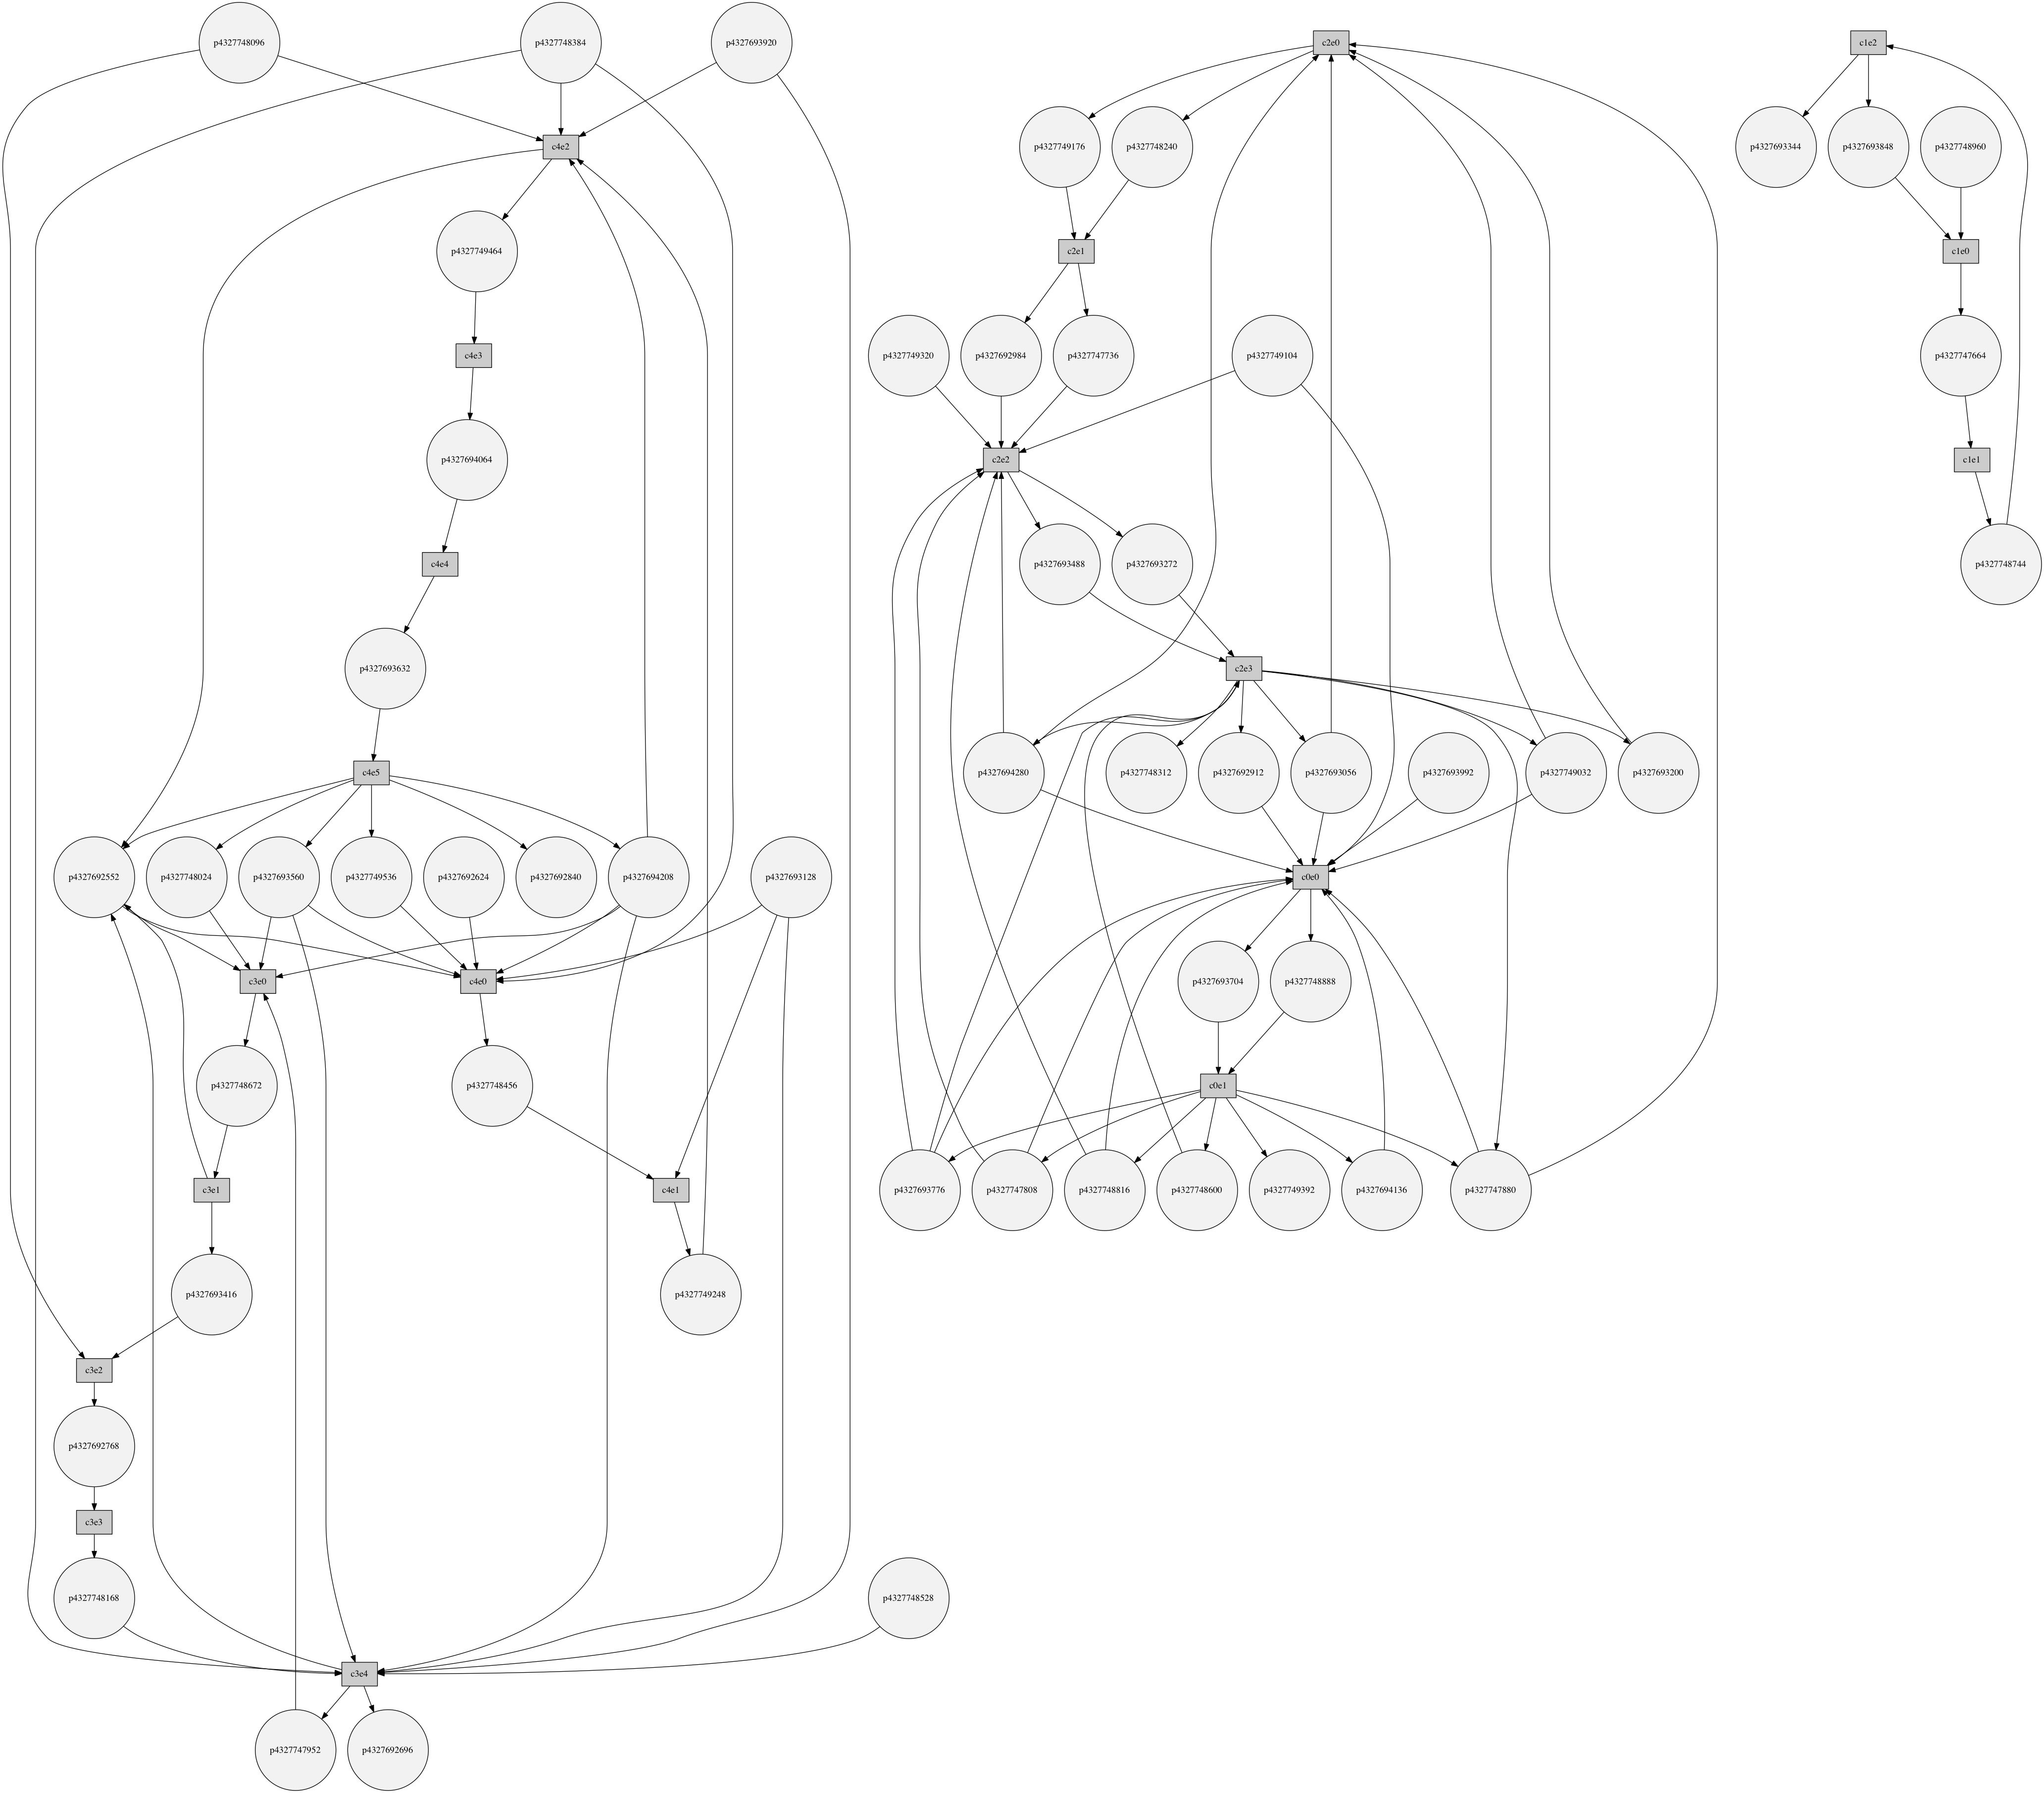
\includegraphics{img/cycles-pol}}}
%%%    \hspace{1cm}
%%%    \subbottom[\label{sfig:allsimp.2}\tiny\textsc{Removal} sobre~\autoref{sfig:allsimp.1}]{\scalebox{.05}{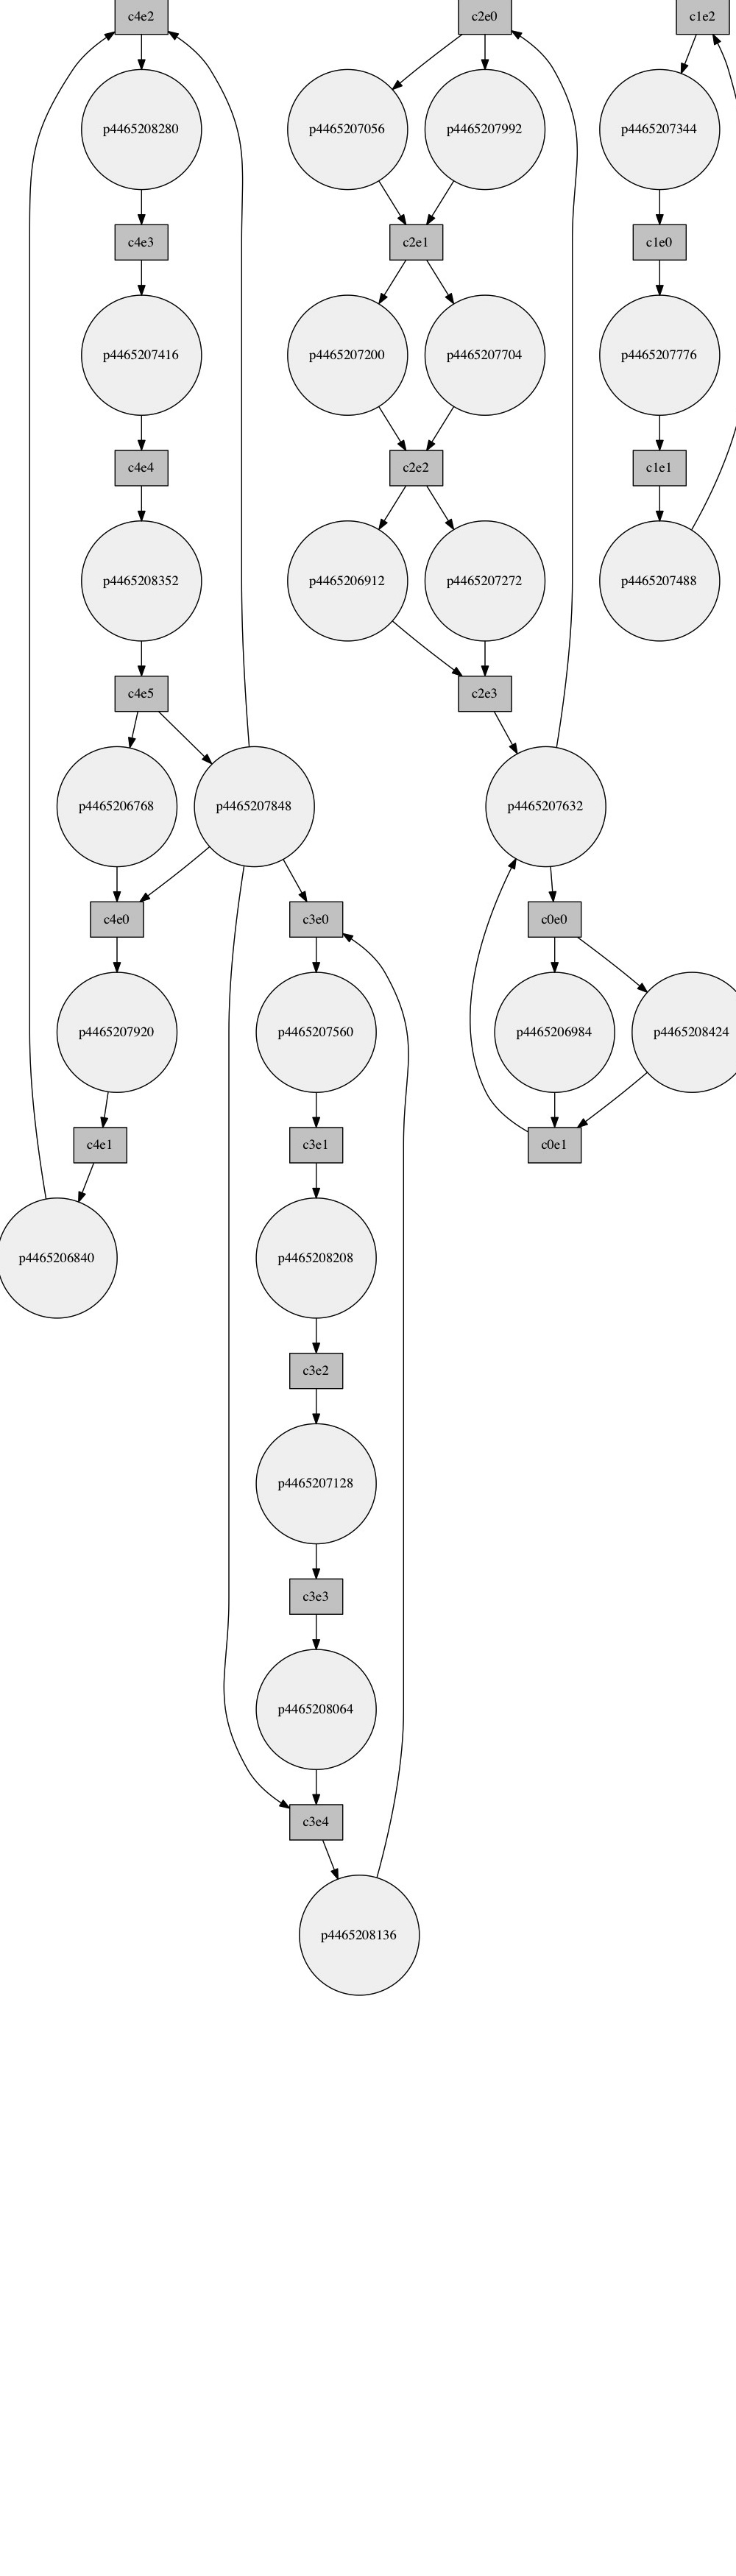
\includegraphics{img/cycles-pol-rem}}}
%%%    \subbottom[\label{sfig:allsimp.3}\tiny Enfoque de~\cite{Murata89}]{\scalebox{.04}{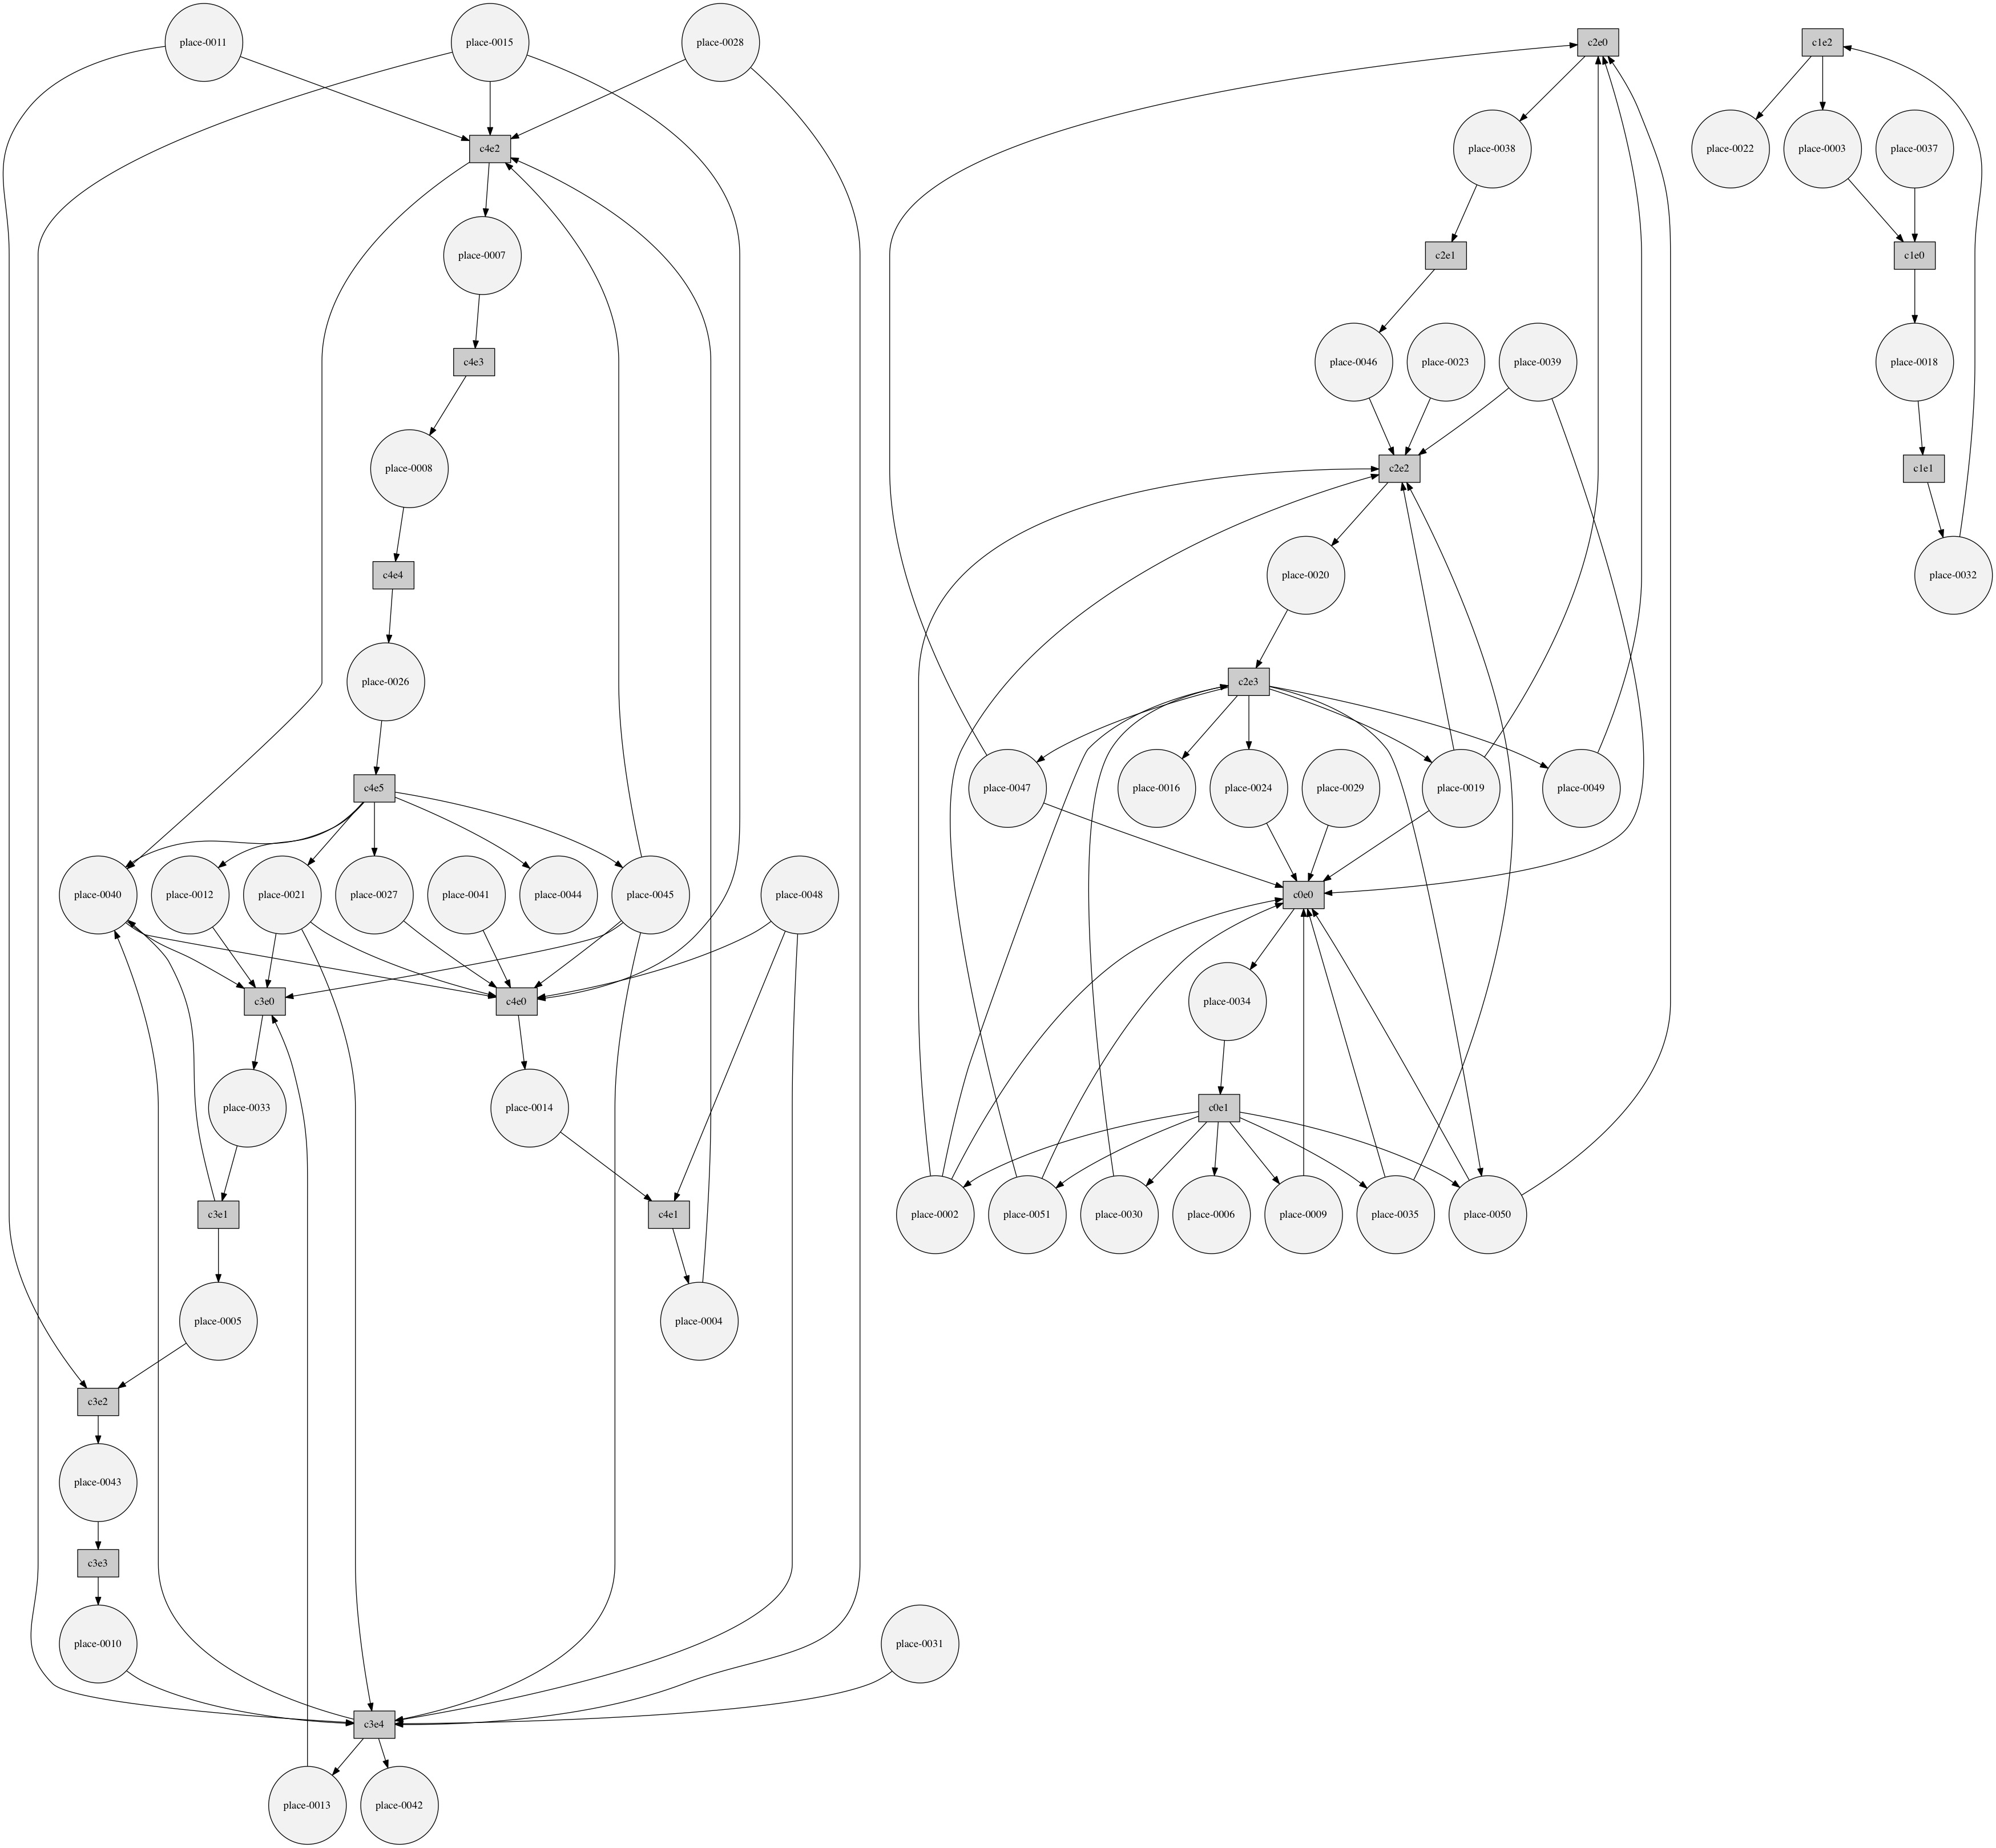
\includegraphics{img/cycles_murata}}}
%%%    \hspace{7mm}
%%%    \subbottom[\label{sfig:allsimp.4}\tiny Enfoque de~\cite{LeonCB15}]{\scalebox{.04}{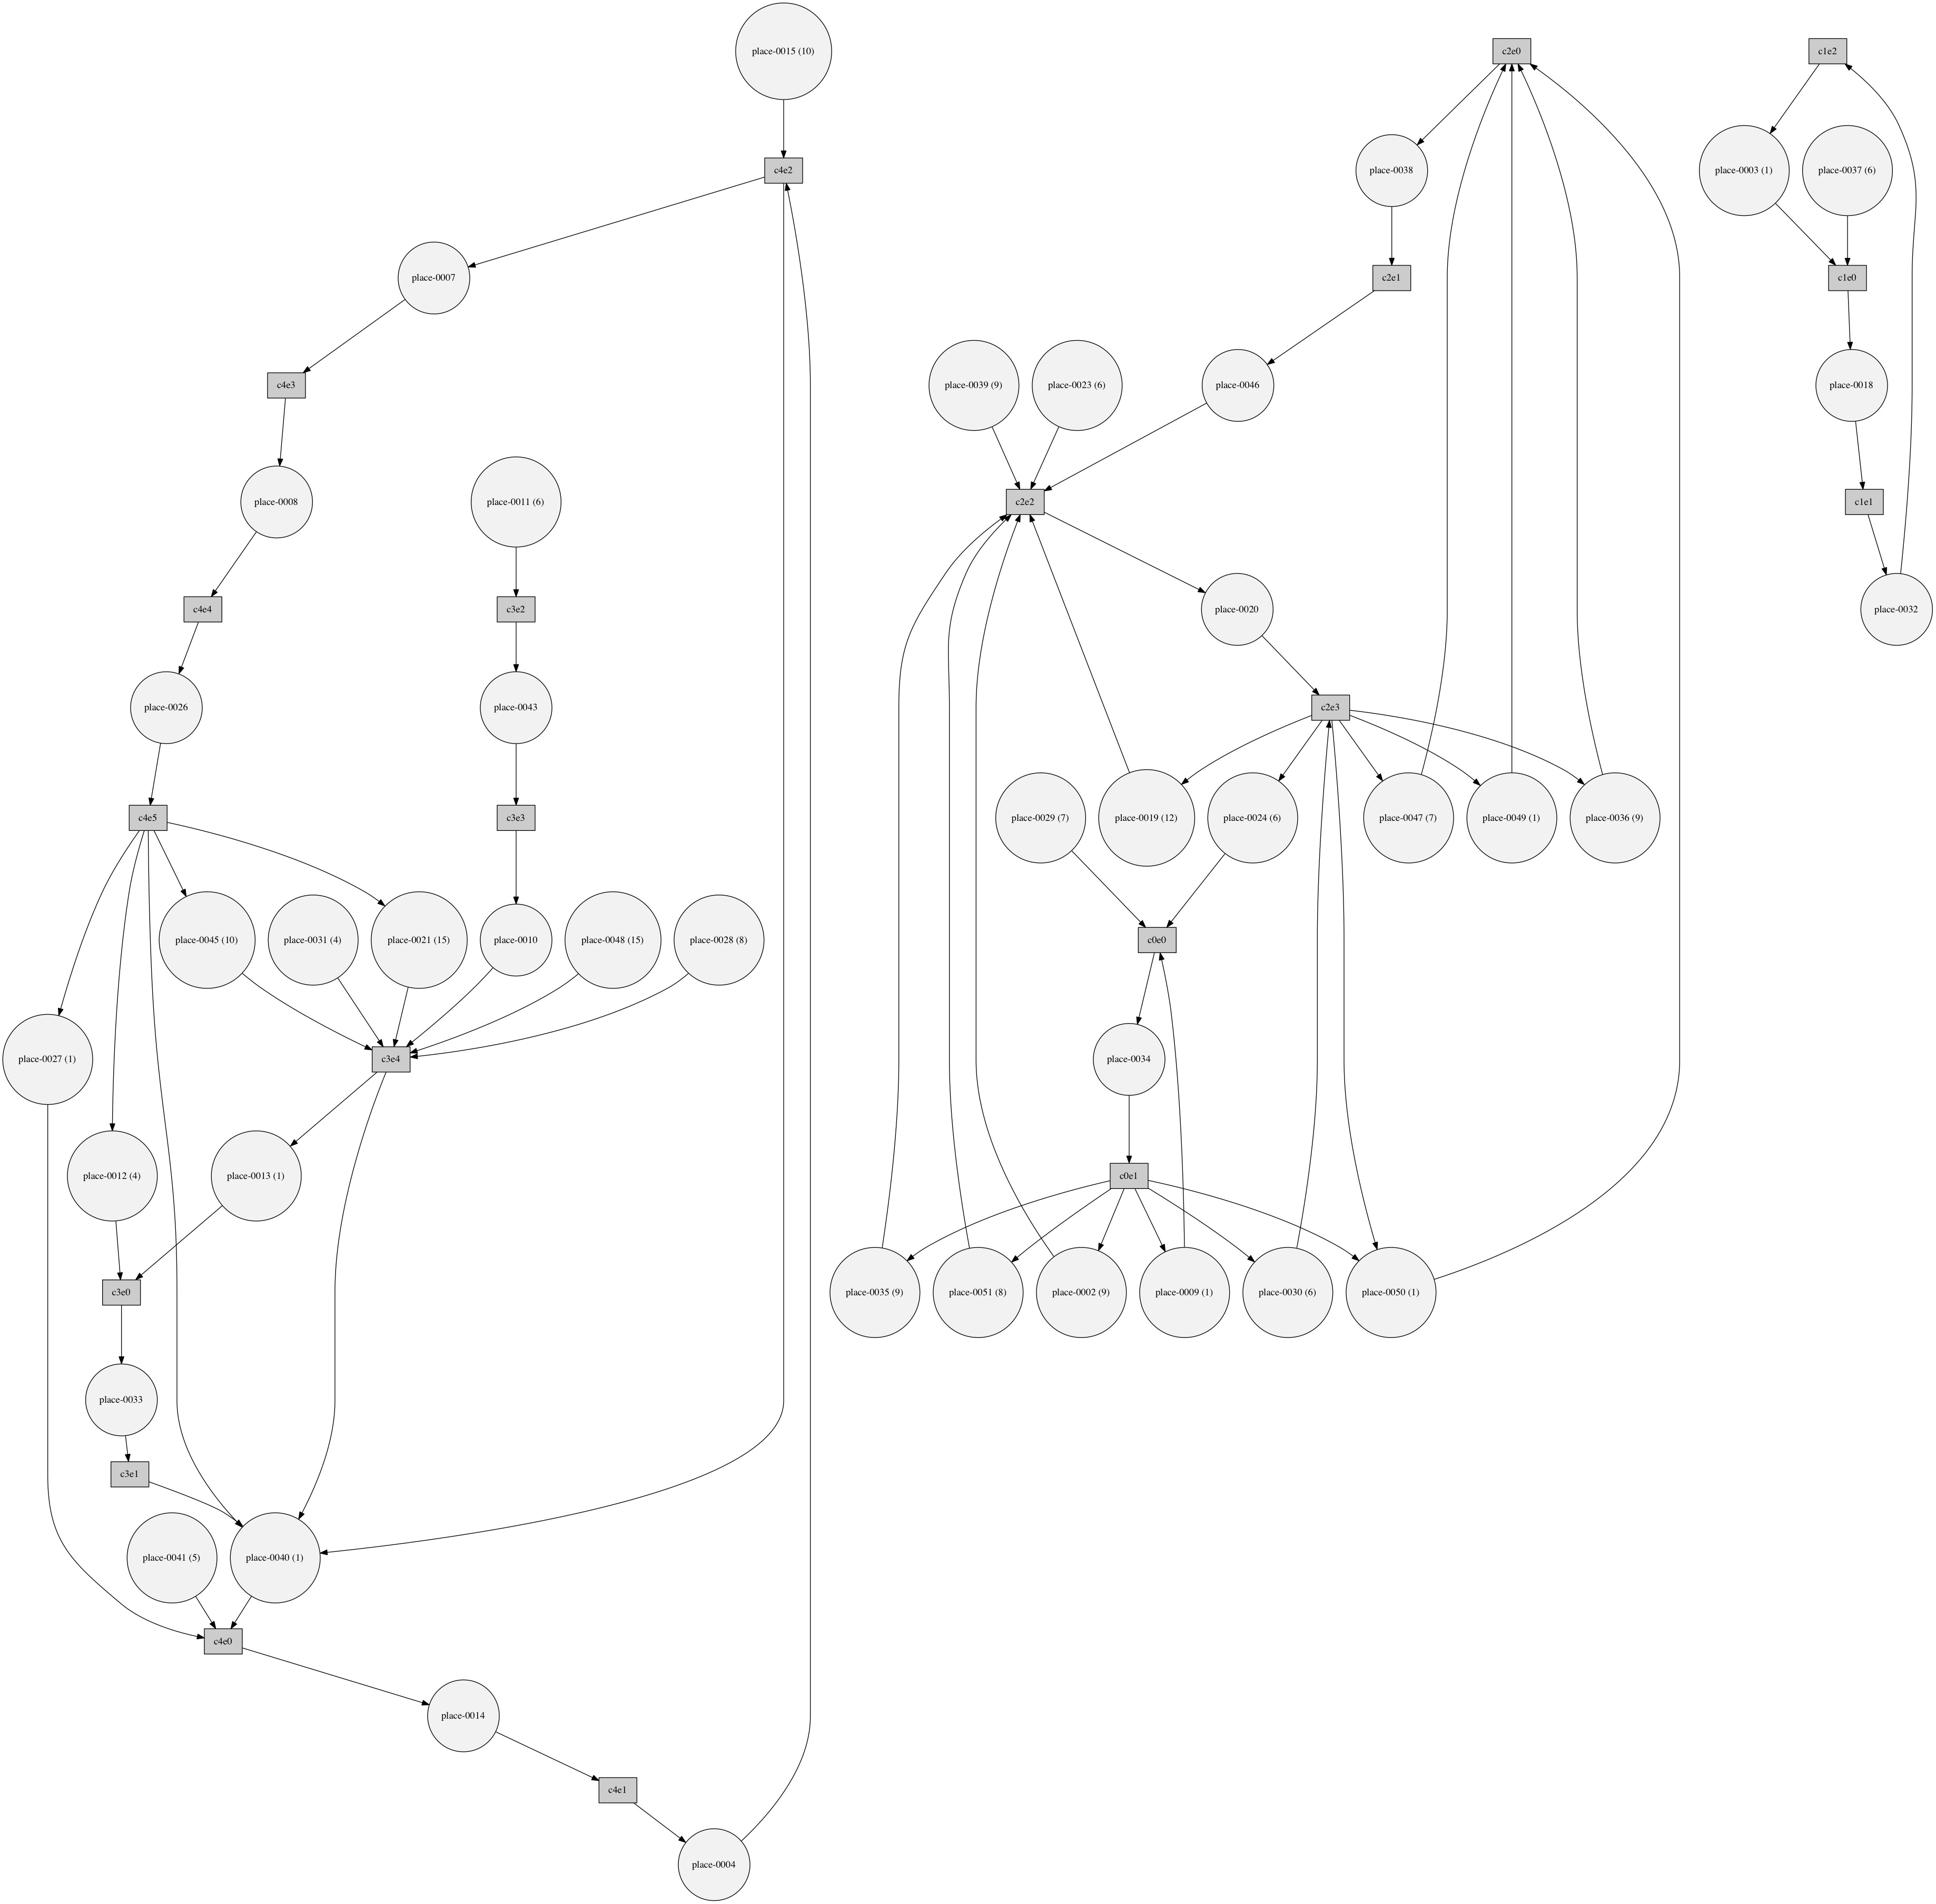
\includegraphics{img/cycles_pnsimp}}}
%%%    \caption{Ejemplo de la aplicación de la técnica presentada.}
%%%\end{figure}

\section{Alcance del trabajo}
\label{sec:alcance}

Esta tesina se plantea como una extensión superadora de los trabajos de Carmona y Cortadella en~\cite{CarmonaC14}
y de León, Carmona y vanden Broucke en ~\cite{LeonCB15}. 
Sin embargo, ambos enfoques poseen algunas restricciones las cuales son heredadas por esta tesina:
los logs de eventos de entrada del procedimiento, deben ser libres de ruido -\textit{noise free}- y las redes generadas
por el proceso se limitan a redes de Petri puras (i.e. aquellas que no contienen ciclos de longitud uno).
Estas restricciones se deben al hecho de que se utiliza teoría de poliedros convexos directamente sobre el log de eventos.

Podrían evitarse estas limitaciones, si se  pre-procesa el log de eventos, filtrando el ruido existente mediante las 
técnicas usuales o bien puede incrementarse artificialmente la longitud de los ciclos de longitud uno evitando los modelos 
no puros. Sin embargo, estos procedimientos escapan del alcance de la tesina y se trabajará considerando las limitaciones
enunciadas.

\section{Estructura de la tesina}
\label{sec:estructura}

En este capítulo se presentaron las motivaciones y los objetivos principales para este trabajo el cual se
plantea como una extensión superadora al trabajo realizado en~\cite{CarmonaC14} y~\cite{LeonCB15}.


Los siguientes capítulos del presente trabajo están organizado de la siguiente manera:

En el ~\autoref{chap:2}, se introducen todas las nociones preliminares necesarias para comprender las contribuciones 
presentadas y plantea una formalización del problema a abordar.

La metodología utilizada para determinar el descubrimiento supervisado de procesos es presentado en el~\autoref{chap:3}, 
en donde se detallan los fundamentos teóricos de la técnica desarrollada y se muestra además, como puede utilizarse para simplificar
y generalizar modelos de procesos arbitrarios.

El~\autoref{chap:4} por su parte, presenta \pachtool, la herramienta desarrollada para esta tesina. Además en este mismo capítulo
se presentan los resultados experimentales de ejecutar \pachtool sobre diferentes benchmark,tanto como una herramienta de descubrimiento
supervisado de procesos así como también utilizándola como herramienta de post procesamiento sobre modelos arbitrarios.

Finalmente en el~\autoref{chap:5} se presentarán las conclusiones de esta tesina y se presetan una serie de posibles trabajos futuros.
